\documentclass {article}
\usepackage{fullpage}

\usepackage{graphicx}
\graphicspath{ {images/} }

\usepackage{hyperref}

\setlength{\parindent}{3ex}

\begin{document}

~\vfill
\begin{center}
\Large

A5 Project Proposal

Title: Windy Awakening

Name: Kevin Haslett

Student ID: 20468033

User ID: kahaslet
\end{center}
\vfill ~\vfill~
\newpage
\noindent{\Large \bf Final Project:}
\begin{description}
\item[Purpose]:\\
	To create a simple game that attempts to replicate the art style of The Legend of Zelda: Wind Waker.

\item[Statement]:\\

The goal of this project to create somewhat of an homage to one of my favourite games.  In particular, I have always loved the art style of Wind Waker, and this project will be an attempt to recreate a number of the most iconic elements of this game.  One of the largest elements of the game, both mechanically, and thematically, is the sailing around the ocean from destination to destination.  Of course another key part of the game is defeating dungeons, but that will be out of the scope for the project.  Because of this I will be focusing solely on creating the nice peaceful sailing experience.

Easily the most iconic visual element of this game is the cell-shaded art style. There is also a very distinctive water texture that needs to be recreated to simulate the look of waves.  Of course in order to convey object detail, we will also need texture mapping.  And shadows are another simple element that adds a lot of depth.  And since Wind Waker is a very bright and colourful game, a bloom filter adds a nice it of polish.  I'd also like to implement a day-night cycle which allows the lighting to change over time.  We'll also need some islands scattered throughout the sea to add some variation amidst the sea, but for the sake of simplicity we will bound the player to their boat, so we don't have to add much detail to the islands.  And finally we'll have some simple boating physics to make the sailing experience somewhat believable.

This project will have a number of interesting challenges associated with.  To begin, I will be implementing it in WebGL, in order make it as accessible as easy to present as possible.  The technical challenges will largely be focused on implementing a variety of different shaders, and combining them in ways to achieve a desired visual effect.

I will learn how to implement a number of different graphics algorithms, and combine them in various ways.  I will also learn a lot about implementing these algorithms in shader code, and how to use frame buffer objects to construct complex final products.  I will also be learning how to use WebGL while completing this project.

\item[Technical Outline]:\\

One of the most complicated aspects of this project will be the water texture.  The goal is to recreate this effect here, from the game:
	
\begin{center}
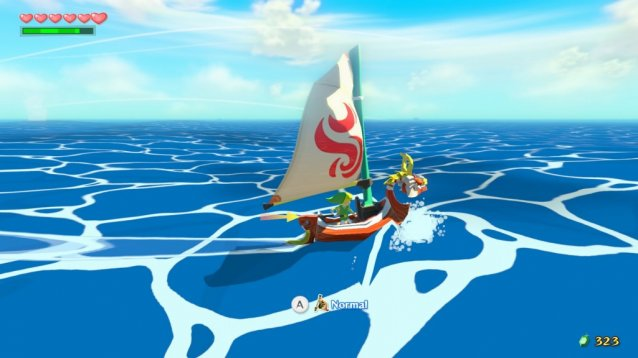
\includegraphics[scale=0.5]{windwaker}
\end{center}

\pagebreak

My plan is to achieve this by first generating a Voronoi diagram (dynamically),  similar to this:

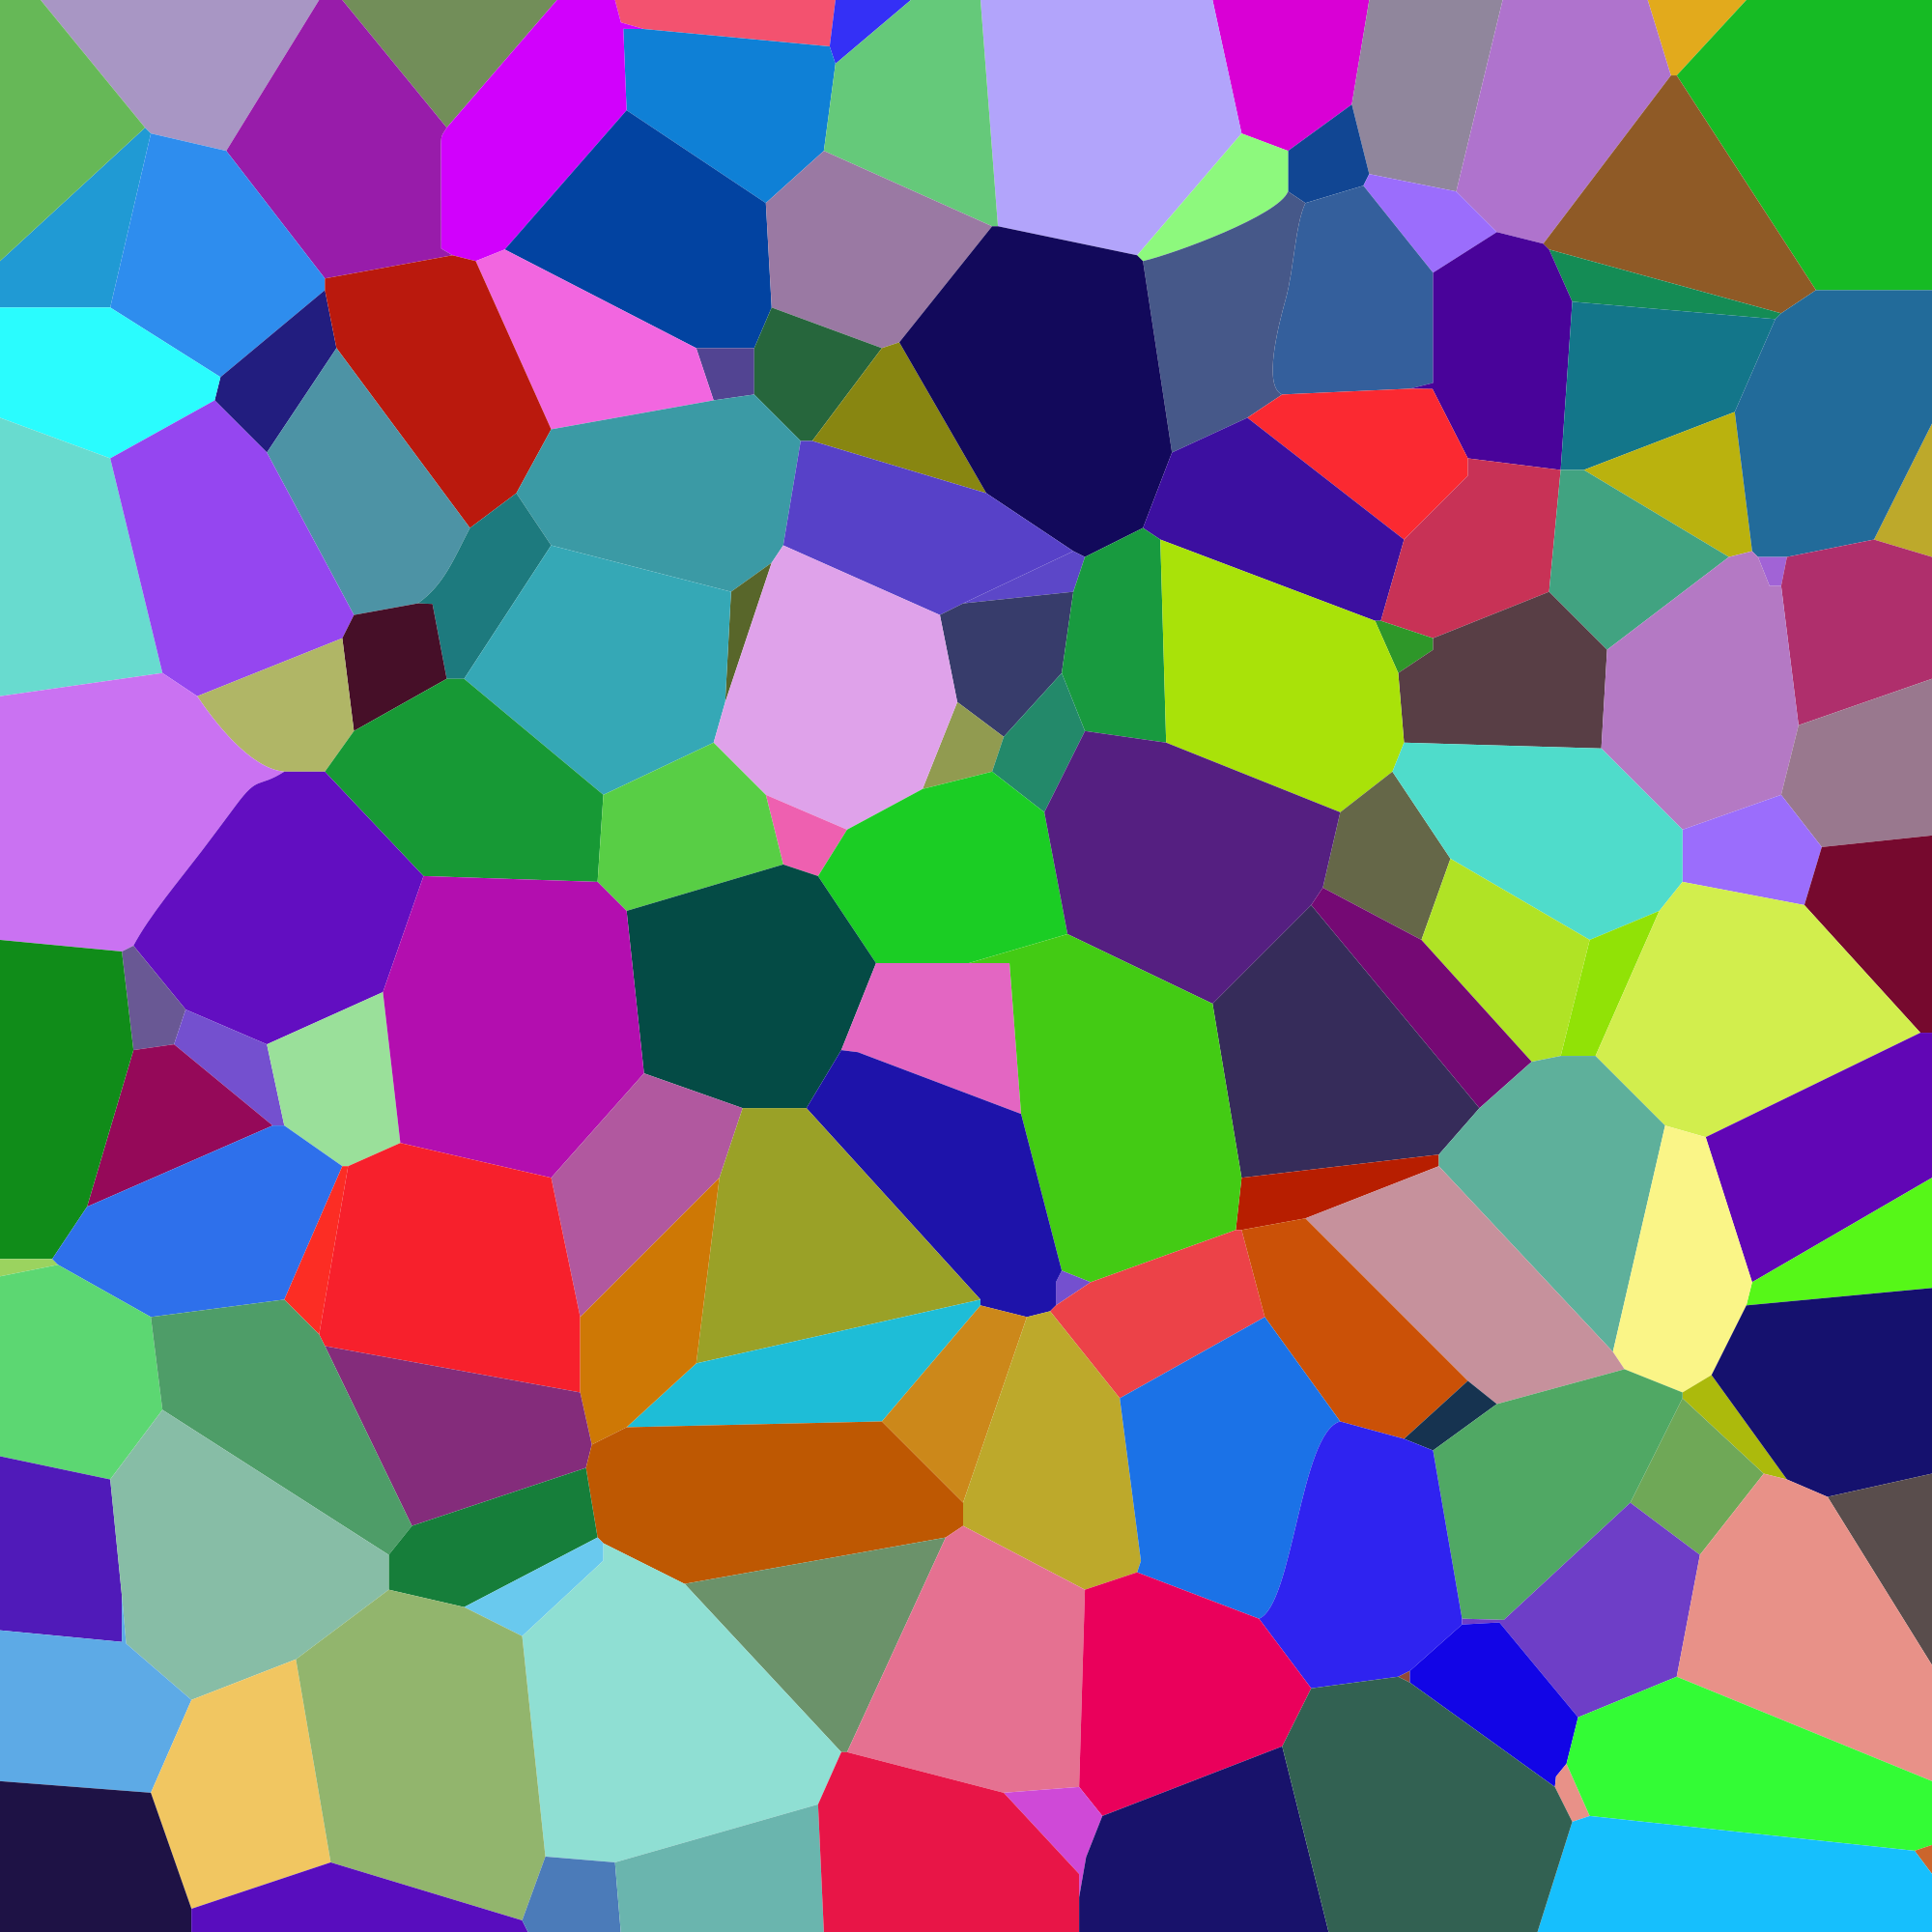
\includegraphics[scale=0.06]{voronoi}

Then we'll apply a Sobel edge detection to highlight only the edges of the regions, producing an image like this:

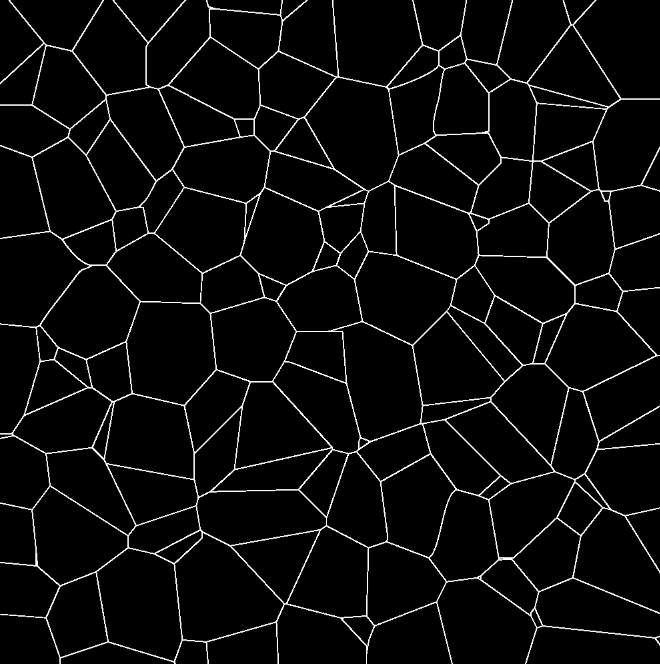
\includegraphics[scale=0.25]{edges}

Then we'll apply some type of blurring algorithm (likely a simple box-blur for efficiency), to round out the edges:

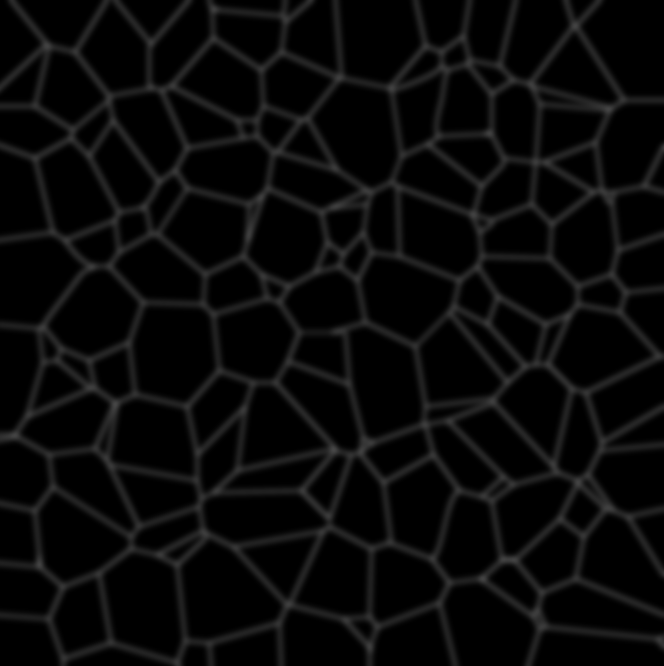
\includegraphics[scale=0.25]{blurred}

And finally, we'll apply a simple threshold mapping, and add the result to a blue image to generate the final water texture:

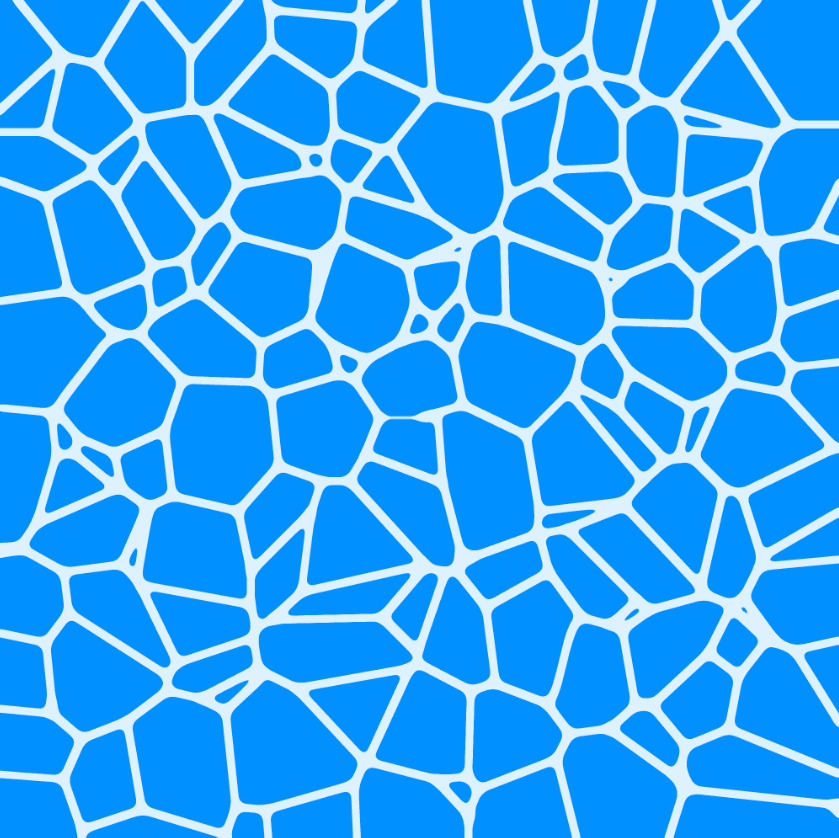
\includegraphics[scale=0.2]{texture}

\pagebreak

These mockups were created using Photoshop as a proof of concept, to demonstrate that this type of image could be generated using a simple enough set of steps that could be replicated in shader code.  Each Voronoi region will slowly move in a random direction so the diagram as a whole will gradually change over time.  The goal is to generate this live so the wave shapes can move over time, assuming it can be done fast enough.  If however this turns out to be too costly, I will settle for a one time generation at runtime.

For the islands, I intend to generate some Perlin Noise to use as a height map for the islands.  It will take some experimenting with thresholds and scaling to determine what works best for convincing islands.  Once I have the height map, I'll simply start with a flat grid of triangles, and use the intensity of the map as the y-value for each point.

I plan to implement a Gooch Lighting model where lighter spots tend to be yellower, and darker spots tend to be more blue.  I will demonstrate this effect by adding a simple day-night cycle, with light direction, and intensity varying over time.

Simple physics to make the motion of the boat through water will be added to attempt some semblance of realism.  Of course I won't be modeling real fluid dynamics, simply an approximation of the boats motion.  I intend to implement a simple dynamics model accounting for a thrusting forward force, and water resistance dragging force that increases with speed. 

I will be supporting texture maps for the scene geometry to allow for much more precise character detailing.  Texture maps should follow a fairly standard thing implementation in WebGL.

In order to save some time, I will be using models from the original Wind Waker game.  These will be of much higher quality than anything I could produce, and won't require the otherwise massive time sink to model and texture things myself.

I will also be implementing shadows, using the common shadow mapping technique for added depth.  Since I intend to rely solely on the Sun as the light source, a directional light will be appropriate.  This will also make the shadow mapping a bit easier, because I will only need to render from the light's perspective once.

For final polish, I'll be implementing cell shading (for the character at least), and a bloom shader to highlight bright spots.  The bloom shader will be able to reuse some of the blurring shader used for the water texture, with a bit of extra effort to selectively blur only the brightest parts of the frame, and add that to the final result.

\item[Bibliography]:\\

A GPU Approach to Voronoi Diagrams,\\
\url{http://nullprogram.com/blog/2014/06/01/}

Edge detection Pixel Shader,\\
\url{http://coding-experiments.blogspot.ca/2010/06/edge-detection.html}

An investigation of fast real-time GPU-based image blur algorithms,\\
\url{https://software.intel.com/en-us/blogs/2014/07/15/an-investigation-of-fast-real-time-gpu-based-image-blur-algorithms}

Implementation of Perlin Noise on GPU An Independent study,\\
\url{http://www.sci.utah.edu/~leenak/IndStudy_reportfall/Perlin%20Noise%20on%20GPU.html}

Soft Shadow Mapping,\\
\url{http://codeflow.org/entries/2013/feb/15/soft-shadow-mapping/}

\end{description}
\newpage


\noindent{\Large\bf Objectives:}

{\bf Full UserID: kahaslet\hfill{\bf Student ID: 20468033}

\begin{enumerate}
     \item[\_\_\_ 1:]  Texture Mapping

     \item[\_\_\_ 2:]  Cell Shading

     \item[\_\_\_ 3:]  Shadow Mapping

     \item[\_\_\_ 4:]  Bloom Shader

     \item[\_\_\_ 5:]  Gooch Lighting Model and Day/Night Cycle

     \item[\_\_\_ 6:]  Voronoi Diagrams

     \item[\_\_\_ 7:]  Edge Detection

     \item[\_\_\_ 8:]  Guassian Blur and Threshold Mapping to Generate Final Water Texture

     \item[\_\_\_ 9:]  Island Terrain Generated Using Perlin Noise

     \item[\_\_\_ 10:]  Simple Sailing Physics
\end{enumerate}

% Delete % at start of next line if this is a ray tracing project
% A4 extra objective:
\end{document}
